A informação aeronáutica que descreve a infraestrutura de um aeródromo, como as dimensões de uma pista e as suas distâncias declaradas, chega aos usuários por meio de produtos oficiais. No Brasil, esses produtos são a Publicação de Informação Aeronáutica (AIP) e as cartas aeronáuticas, publicadas pelo Departamento de Controle do Espaço Aéreo (DECEA). Eles são atualizados por emendas, segundo o ciclo AIRAC, e cada nova edição substitui a anterior. O que o usuário recebe, portanto, é o estado dos dados na data de efetividade de cada produto.

Os Procedimentos para os Serviços de Navegação Aérea -- Gestão da Informação Aeronáutica (PANS-AIM) estabelecem requisitos de qualidade para esses dados, entre eles a integridade e a rastreabilidade, além de também exigir consistência entre os produtos de informação aeronáutica \cite{icao2018pansaim}. Esses requisitos se aplicam à cadeia de produção da informação, contudo, o produto publicado, apresenta os valores sem o registro das alterações que os produziram.

O Aeroporto de São José dos Campos (SBSJ) ilustra essa situação. Duas cartas do aeródromo apresentam valores diferentes para o comprimento da pista, a zona de parada (\textit{stopway}, SWY), as dimensões da faixa de pista e a distância disponível para aceleração e parada (ASDA) da cabeceira~16 (Figura~\ref{fig:adc-aoc}). A primeira é a Carta de Obstáculos de Aeródromo (AOC), publicada na emenda AIRAC~2213, de 2022 \cite{decea2022aoc} e a segunda é a Carta de Aeródromo (ADC), publicada na emenda AIRAC~2604, de 2026 \cite{decea2026adc}. Na AOC, as distâncias declaradas correspondem a uma pista de 2676~m e a uma ASDA de 3001~m para a cabeceira~16 (Figura~\ref{fig:aoc-dist}) e a planta da mesma carta indica uma SWY de 325~m e uma faixa de $3121 \times 300$~m (Figura~\ref{fig:aoc-planta}), enquanto na ADC (Figura~\ref{fig:adc}), os valores correspondentes são 2675~m, 2958~m, 283~m e $3118 \times 280$~m.

\begin{figure}[htbp]
    \centering
    \begin{subfigure}{\linewidth}
        \centering
        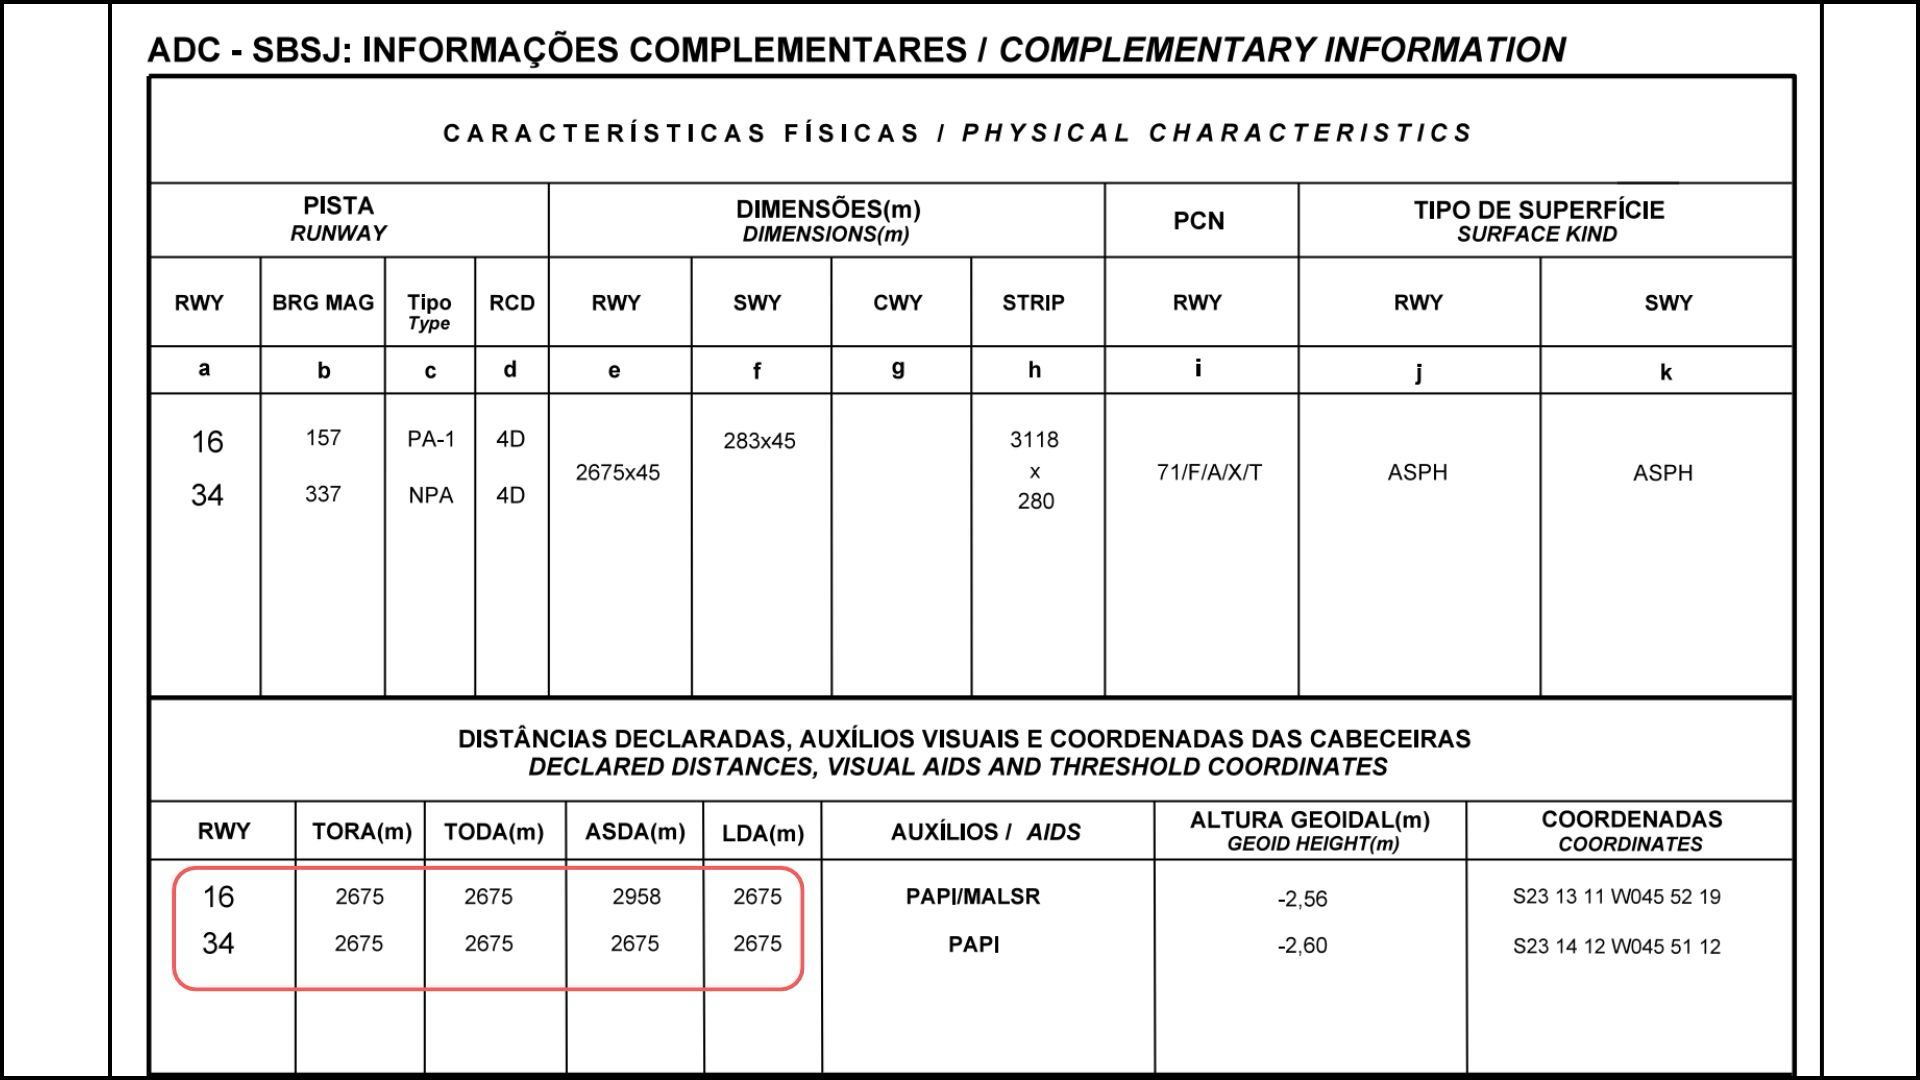
\includegraphics[width=0.9\linewidth]{Figures/ADC_SBSJ.png}
        \caption{ADC, emenda AIRAC 2604 (2026): informações complementares.}
        \label{fig:adc}
    \end{subfigure}

    \bigskip
    \begin{subfigure}{\linewidth}
        \centering
        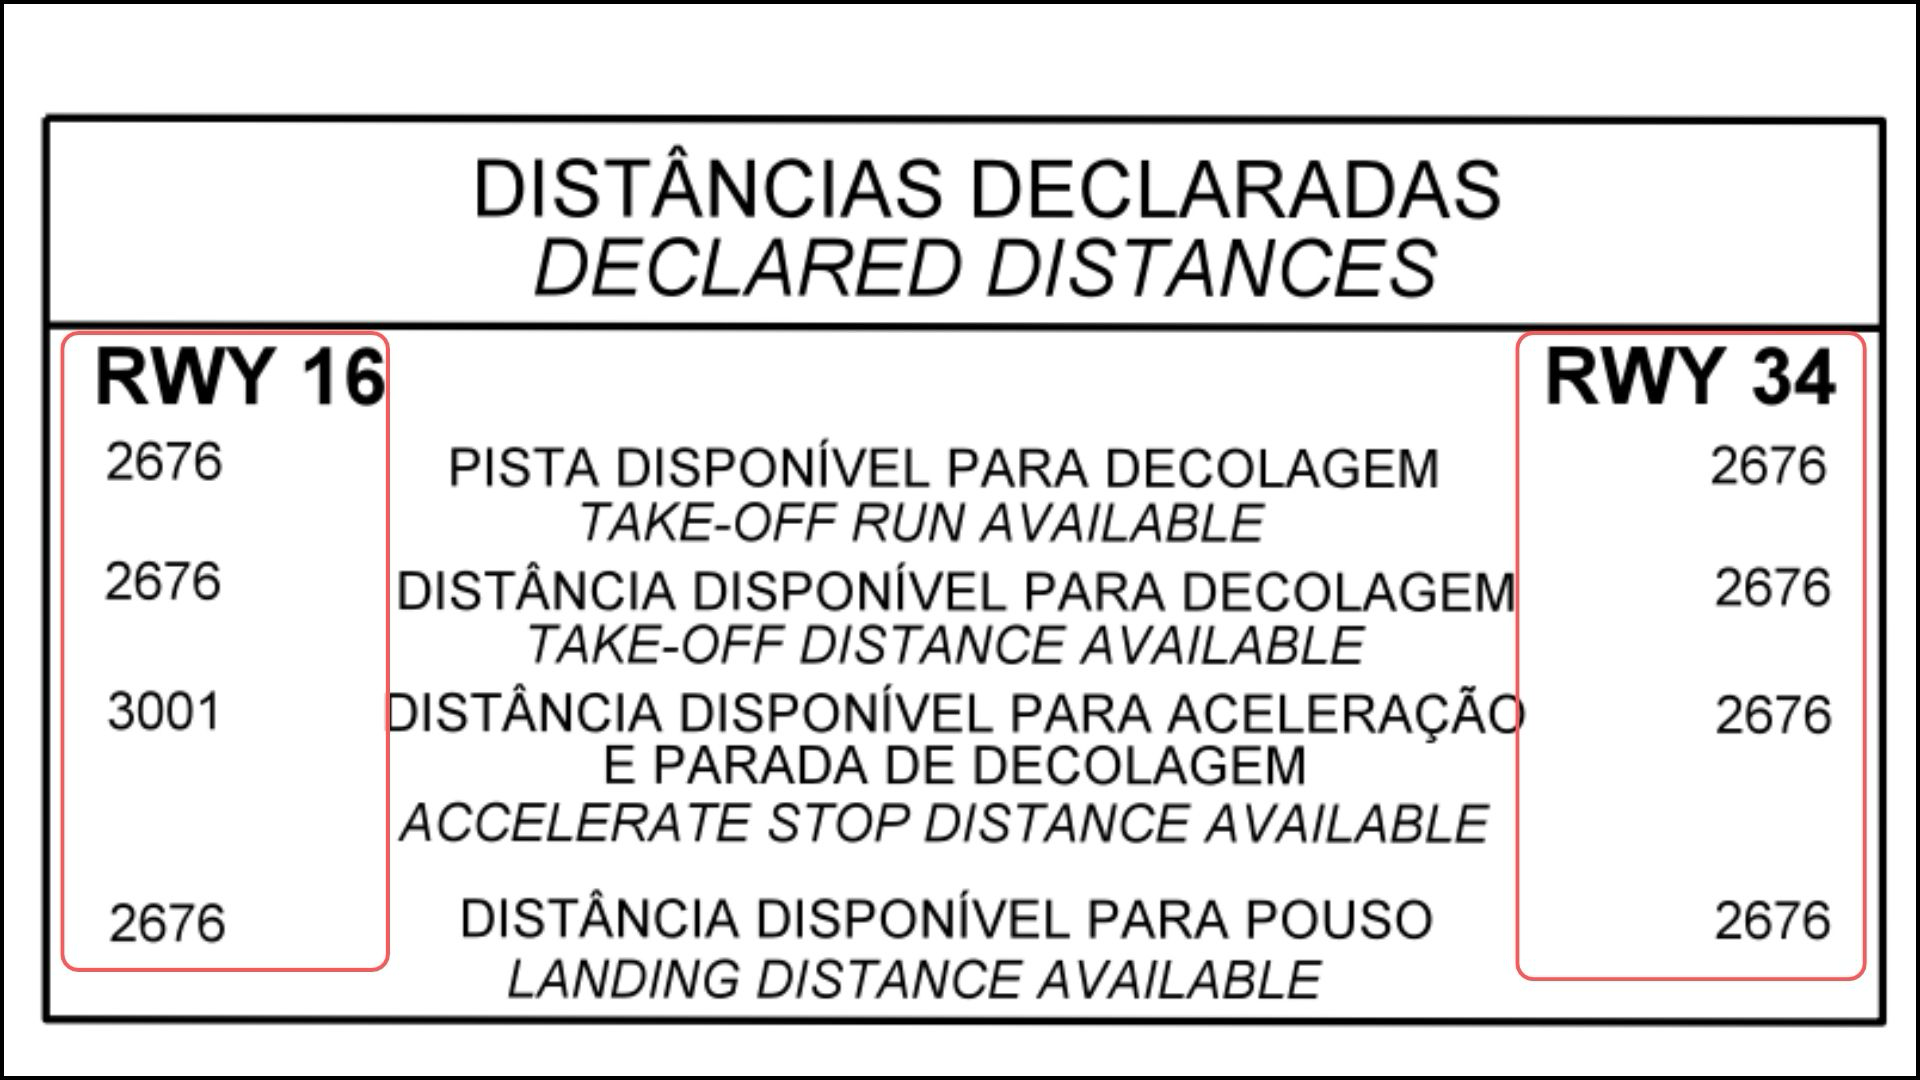
\includegraphics[width=0.5\linewidth]{Figures/AOC_SBSJ_pista.png}
        \caption{AOC, emenda AIRAC 2213 (2022): distâncias declaradas.}
        \label{fig:aoc-dist}
    \end{subfigure}

    \bigskip
    \begin{subfigure}{\linewidth}
        \centering
        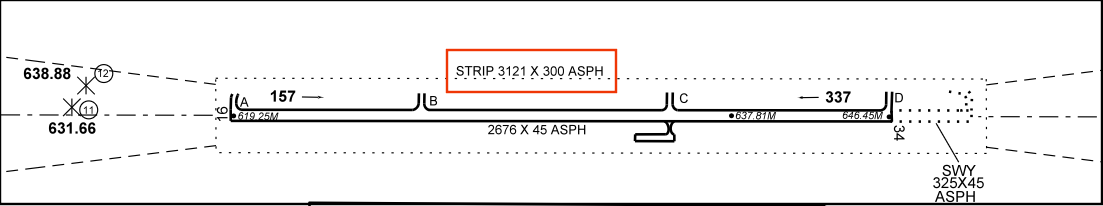
\includegraphics[width=0.9\linewidth]{Figures/AOC_SBSJ_distancia_declarada.png}
        \caption{AOC, emenda AIRAC 2213 (2022): dimensões em planta.}
        \label{fig:aoc-planta}
    \end{subfigure}

    \caption{Dimensões e distâncias declaradas da pista do SBSJ em duas cartas
    oficiais.}
    \label{fig:adc-aoc}

    \medskip
    {\small Fonte: DECEA, AIP Brasil (cartas completas nos Anexos~\ref{anexo:adc}
    e~\ref{anexo:aoc}).}
\end{figure}

A divergência pode decorrer, em parte, de as duas cartas terem propósitos distintos. Enquanto a AOC reúne as informações sobre obstáculos necessárias ao cálculo de desempenho na decolagem, a ADC apoia a movimentação das aeronaves no aeródromo \cite{icao_anexo4}. Além disso, foram emitidas com quatro anos de intervalo e, nesse período, podem ter ocorrido novos levantamentos, obras na pista, correções ou mudanças nos critérios de cálculo. A prática de adotar a publicação mais recente como vigente é, nesse contexto, adequada.

Nenhum dos documentos informa o que motivou a alteração, quem a realizou ou de quais medições e critérios os novos valores dependem. Esse conhecimento possivelmente existe no órgão responsável pelas publicações, mas não acompanha os dados publicados. Além disso, reconstruir o que estava publicado em uma data passada depende de que o usuário tenha conservado a edição correspondente. No caso do SBSJ, a comparação só foi possível porque ambas as cartas permaneciam disponíveis.

O problema abordado neste trabalho é, portanto, de rastreabilidade. Busca-se garantir que, para qualquer valor publicado, seja possível:
\begin{itemize}
    \item identificar a sua origem, as premissas de que depende e a causa de cada alteração;
    \item reconstruir o estado dos dados em qualquer instante;
    \item verificar que esse histórico não foi modificado.
\end{itemize}

Para tratar esse problema, este trabalho propõe uma arquitetura de dados em que cada alteração é registrada como um evento imutável, com autor e causa declarados. Os valores que podem ser calculados a partir de outros, como comprimentos e distâncias declaradas, não são armazenados: são derivados das premissas no momento da consulta. O princípio é o mesmo dos registros contábeis, em que nenhum lançamento é apagado e um erro é corrigido por um novo lançamento, com motivo declarado \cite{helland2016}. Os fundamentos dessa abordagem e a sua relação com os modelos de informação aeronáutica existentes são apresentados no Capítulo~\ref{chap:fundamentacao}.

\section{Objetivos}

Este trabalho busca responder à seguinte pergunta:

\begin{quote}
Em que medida uma arquitetura baseada em \textit{event sourcing} torna auditáveis os dados geolocalizados de infraestrutura aeroportuária, e quais são os limites dessa auditabilidade?
\end{quote}

A hipótese é que essa arquitetura permite que tais dados sejam:
\begin{itemize}
    \item rastreáveis até a sua causa;
    \item recalculáveis a partir das premissas;
    \item reconstruíveis no tempo;
    \item consistentes entre produtos;
    \item protegidos por evidência de adulteração.
\end{itemize}
Os limites da auditabilidade não são presumidos: resultam dos experimentos e das restrições declaradas pela própria implementação.

\subsection{Objetivo geral}

Propor e avaliar uma arquitetura de dados baseada em \textit{event sourcing} que torne auditáveis os dados geolocalizados de infraestrutura aeroportuária, identificando os limites dessa auditabilidade. O escopo restringe-se à estrutura física de uma pista, embora a arquitetura admita extensão a dados operacionais.

\subsection{Objetivos específicos}

\begin{itemize}
    \item Caracterizar a lacuna de rastreabilidade nas publicações aeronáuticas, a partir das diferenças entre as cartas oficiais do SBSJ e dos requisitos do PANS-AIM.
    \item Propor uma arquitetura em que cada alteração seja registrada como evento imutável, com autor e causa declarados e encadeado por \textit{hash}. Nela, a geometria é representada pelas premissas que a geram, e os valores derivados são calculados no momento da consulta.
    \item Implementar a arquitetura como biblioteca de código aberto, independente do experimento que a avalia.
    \item Avaliar a arquitetura por meio de seis experimentos sobre a pista do SBSJ, com dados reais, cada um dedicado a uma propriedade e com critérios de aprovação definidos antes da execução.
    \item Identificar os limites da auditabilidade obtida, distinguindo o que os experimentos demonstram do que é apenas argumentado.
\end{itemize}

\section{Organização do trabalho}

O Capítulo~\ref{chap:fundamentacao} apresenta os fundamentos em que o trabalho se apoia, isto é, os padrões de informação aeronáutica e geoespacial e os modelos de dados que retêm histórico, em especial nos sistemas financeiros. O Capítulo~\ref{chap:metodologia} descreve o método, com os requisitos que a solução deve atender, o estudo de caso e os experimentos que a avaliam. O Capítulo~\ref{chap:solucao} desenvolve a arquitetura proposta, a sua implementação e a sua aplicação ao SBSJ. O Capítulo~\ref{chap:resultados} apresenta os resultados dos experimentos, e o Capítulo~\ref{chap:discussao} os discute, junto com os limites identificados. O Capítulo~\ref{chap:conclusao} apresenta as conclusões e os trabalhos futuros.
